% \subsubsection{Overview}
% \label{sec:entity-schema-overview}

The entity schema 
of a \UTP{} instance
combines
a hierarchy of course elements %namely, 
(i.e., courses, course parts, part classes and class sessions)
a scheduling horizon over which sessions are to be scheduled,
and 4 types of resources to which sessions must be allocated to
(i.e., rooms, teachers, students and student groups).
The schema encodes the nesting of course elements
and various properties and constraints 
concerning 
session scheduling,
resource availability, 
resource eligibility,
teaching service,
room capacity,
and student sectioning. %\todo{be more specific on sectioning? ie. out of scope}
% Session-related properties and constraints are either specified on individual sessions
% or inherited from course parts.
% All constraints are ultimately cast as domain, cardinality or assignment constraints on decision variables
% in the core model.

The scheduling horizon is a range
%$\SLOT$ 
of integers denoting \timepoints{}.
The \timepoints{} are the start and end times allowed for sessions
and any duration (i.e., session length, travel time and break time)
is measured as a number of \timepoints{}. 
The horizon is
defined using 3 instance fields: 
the number of weeks $\week$ dividing the horizon, 
the number of weekdays $\weekday$ making a week 
and the number of daily slots $\dailyslot$ making a 24-hour day.
The \timepoints{} correspond to all possible triplets combining a week, a weekday, and a daily slot. 
Note that daily slots may have any granularity (e.g., 1 minute, 2 hours)
and
%Besides, 
the scheduling horizon may be sparse
(e.g., if weeks $i$ and $i+1$ are not consecutive calendar weeks for some $1\leq i<\week$ 
or if weekdays are dropped, i.e., $\weekday<7$).
%If so, any duration exceeding a day or a week should be interpreted with care.

Course elements follow a hierarchical structure.
% nesting
% courses,
% %(set $\COURSE$),
% course parts,
% %(set $\PART$),
% part classes,
% %(set $\CLASS$),
% and class sessions.
% %(set $\SESSION$).
% %(\hyperref[feat:coursehierarchie]{``course hierarchy''}), 
Each course (e.g., Algorithms) consists of one or more parts (e.g., Lecture and Lab),
each part is taught to one or more classes (e.g., lecture classes A and B),
and all classes of a part have the same number of sessions (e.g., sessions 1 to 10 for each lecture class).
% The classes of a part share the same number of sessions.
%TODO \todo{@corentin: post-soumission, toutes les règles/assertions du schéma (eg. les classes d'1 part doivent avoir la même durée, inclusion entre required/possible, ordre en min/max) sont à compiler dans une section séparée de l'annexe.}
~The schema requires that all sessions in a class have the same duration
and be chronologically ranked,
i.e., session of rank $i+1$ in a class must start after session of rank $i-1$ ends in any solution.
These constraints are paramount to model course plans that rely on clear-cut sessions
(e.g., starting lab classes after 2 lecture sessions,
synchronizing the $5^{th}$ sessions of lab classes for a joint examination).
Besides, the schema allows to restrict the possible time slots for the sessions of a part
by setting allowed and forbidden ranges using the time format.
%Note that sessions are considered uninterruptible 
%and %, in particular, 
%may not overlap 2 days.
Note that 
sessions must start and end on the same day, and cannot be interruptible. % and cannot extend over two days.
%
The schema also specifies a set of possible resources for each session.
As for students, % and groups, 
a sectioning plan
%\footnote{Student sectioning consists in generating and matching student groups with classes consistently with course enrollments of students, class headcount thresholds and group sectioning policies (e.g., aggregating groups bottom-up from labs to lectures) or cross-course constraints (e.g., populating classes of different courses of a curriculum with identical groups).}
%\todo{comment-out footnote?}
is assumed and hard-coded together with group-to-class assignments.
Specifically, 
students are partitioned into groups,
and groups aggregated and assigned to classes
with no group being assigned to more than one class per course part.
The schema encodes group and class headcounts
as well as class headcount thresholds used for sectioning.%TODO \todo{@corentin: thresholds really needed in the models? Dicussion en réunion le size et le headcount en fonction du mode de fonctionnement }
~Other sectioning data and constraints %(e.g., course enrollments, group aggregation rules) 
are compiled away.
%but remains necessary for ...}
The implicit constraint to satisfy %to satisfy here %enforced on groups %enforced by the entity model 
is that a group must attend all the sessions of a class it is bound to.
%(\hyperref[feat:group]{``group''}). 

% As opposed to students, % and groups, 
Teacher-to-session assignments are not fixed
but subject to domain and cardinality constraints.
To meet practical needs, 
the schema allows multiple teachers per session
(e.g., joint supervision of a lab session) %, exam requiring several monitors)
and %as well as 
teacher-less sessions 
(e.g., unsupervised project work).
The number of teachers per session is specific to each course part
and is lower- and upper-bounded, possibly fixed.
Each part is also associated with 
a set of required teachers
and a superset of allowed teachers.
Hence two sessions of a class may be allocated different teachers and numbers of teachers.
A part also sets the fixed number of sessions a teacher is committed to.
% Again, this number may be fixed or bounded.
Overall, various demand and capacity requirements relating to teaching service 
can be addressed on course parts.
If needed, finer-grained rules may be imposed
(e.g., requiring the same staff for a class, naming a lecturer for a session).

Similarly, each part sets the required and possible rooms for its sessions and their number.
This caters for the case of multi-room sessions (e.g., for hybrid teaching)
and room-less sessions (e.g., field trips). %\todo{english SORTIE}
In addition, each part casts its sessions as room-exclusive or room-inclusive
which entails different allocation constraints.
A session is room-exclusive if none of the room(s) hosting it may simultaneously host another session.
Conversely, a room-inclusive session allows for its room(s) to be shared from start to finish.
While single-room sessions may be cast as exclusive or inclusive,
multi-room sessions may only be cast as exclusive.
That is, every session of a part whose room upper-bound is greater than 1 is considered exclusive. 
The rationale is that multi-room inclusive sessions have arguably little practical interest %in the timetabling domain.
and they also burden the computational model with decisions to make on the distribution of groups in shared rooms. 

All resources enforce capacity constraints w.r.t. their utilization.
%Since modalities differ from one environment to the next, 
Students, teachers and rooms are considered cumulative resources in this respect.
That is, they may attend, teach or host simultaneous sessions.
A cumulative model is paramount 
to satisfy flexible attendance requirements
(e.g., students attending tutoring sessions overlapping with compulsory courses)
and multi-class events 
(e.g., an amphitheater hosting %simultaneous exams or 
a joint conference for different classes).
Again, rules may be used to impose disjunctive resources 
or to ban session overlapping.
%
No limit is set on the number of parallel sessions teachers and students may attend.
Session hosting however is subject to capacity constraints
and the schema encodes the capacity of each room,
allowing for infinite capacity to handle virtual rooms. %\todo{@corentin: is the virtual room case covered in the models?} marc: oui
As discussed above, 
at any point in time, 
an allocated room will
either 
co-host a multi-room (exclusive) session
or host one or more single-room sessions (one only if a session is exclusive).
The schema hence enforces two kinds of capacity constraints.
The single-room case involves checking
if the total headcount of the session(s) falls below the room capacity.
The multi-room case involves
ensuring the total capacity of the rooms envisaged for the session exceeds its headcount.
If so, 
%As discussed above, 
no restriction is imposed as to the distribution of students in rooms
and whether it preserves group structure or not.

Lastly, the schema provides users with the ability to define their own classes of entities,
mixing course elements and resources as needed
with no limit on classification
(e.g., a block of rooms, the lecturers of a faculty department).
This is achieved by labeling entities.
Labels, built-in entity types and ids
are the building blocks of the query language
to forge rules for any group of entities.



% Similarly to the {\ITC} language, 
% the {\UTP} language adopts a multi-scale schedule horizon (i.e., weeks, weekdays and daily slots), a mixed set of resources (i.e., students, student groups, rooms and lecturers), and a hierarchical course structure (i.e., course parts, part classes and class sessions). In our approach however, class sessions (a.k.a., class meetings) are considered as first-class objects that must be scheduled individually alongside resources. 
% The model supports single-resource sessions (e.g., single lecturer) as well as multi-resource sessions (e.g., hybrid teaching), and encodes core constraints relating to student sectioning, session scheduling and resource allocation. %which are cast using built-in properties and relations over entities (i.e., resources and course elements) and sessions. 
% All resources are assumed cumulative (i.e., rooms, lecturers and students may host, teach and attend overlapping sessions) but this policy may be overridden with disjunctive scheduling rules.
% The rules language effectively allows to enforce additional constraints on selected sets of sessions and entities (i.e., resources and course elements).
% Rules are expressed using a catalog of timetabling predicates and a comprehension syntax to group, filter and bind sessions and entities. 
% Specifically, each rule denotes a conjunction of \UTP{} constraints sharing the same predicate (e.g., periodicity of all lecture classes of a course) and constraints are technically generated through a rule flattening process. %on selected classes of entities and sessions 

% %Specifically, the sessions of a course part are cast as single-resource (e.g., face-to-face lectures) or multi-resource sessions (e.g., hybrid sessions) by quantifying the needed resources. 
% %Lecturers and rooms are distributed over course parts while students are distributed over courses based on registrations which determines the resources allowed for each session.
% %%The resources allowed for a session follow from the distribution of student registrations over courses and that of lecturers and rooms over course parts. 
% %The volume of sessions per student depends on individual course registrations as class attendance is compulsory; it is configurable per lecturer in each course part but is unconstrained for rooms. 
% %%The volumes of sessions are configurable per teacher in each part (i.e., sessions quota) but pre-determined for students (i.e., class attendance is mandatory) and unconstrained for rooms. 
% %No limits apply on simultaneous resource usage but for rooms whose hosting capacity must match class size. Any resource may hence be allocated to joint or overlapping sessions  (e.g., lecture and optional tutoring for students) except for rooms hosting multi-room sessions. In any case, rules may be enforced as needed to prevent sessions from overlapping or to make resources fully disjunctive. As for session scheduling, start time grids are configurable in each course part and the model simply requires full session sequencing in each class. Lastly, the model sections students into classes and supports subgroup inclusion constraints between classes. Note that student groups are considered a by-product of student sectioning and as such may only be listed in the solution component. 

% %The rules language allows to state additional constraints using a catalog of timetabling predicates. A rule is tied to a predicate and models a conjunction of constraints on selected classes of entities and sessions (e.g., disjunctive scheduling rule for lecturers, temporal constraints on the courses of a curriculum). Each constraint applies to one or more pairs, called e-maps, and may involve parameters based on the predicate signature. An e-map either associates a resource with a subset of its compatible sessions or a course element with a subset of its constitutive sessions. In the first case, the e-map is interpreted as a set of conditional entity-to-session assignments while it is unconditional if it models a course element. Specifically, a constraint is only evaluated on the sessions for which its e-map argument(s) and the considered solution propose the same entity. Each predicate may be applied equally well to any type of e-map and be used to constrain resources (e.g., lecturer unavailability), course elements (e.g., class periodicity) or individual sessions (e.g., session parallelization). %Note that constraints on e-maps modeling sessions of course elements are de facto unconditional. 
% %Formally, a rule is defined by a universally quantified formula wherein quantifiers restrict the domains of the e-map variables. A language of selectors is provided to build and filter domains of e-maps based on session ranks, entity identifiers, entity types, or any user-defined class of elements (e.g., team of lecturers, block of rooms). A rule hence denotes the conjunction of constraints obtained by instantiating the predicate over the cross-product of the domains of the e-map variables. 

% \todo{david toolchain figure? uncomment}
% % \begin{figure}
% %     \centering
% %     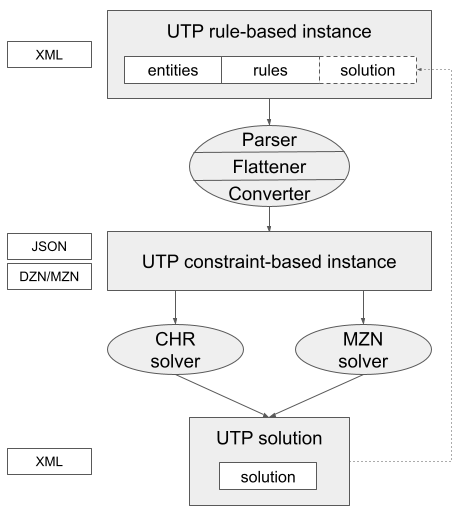
\includegraphics[scale=0.4]{img/utp_toolchain.png}
% %     \caption{The \UTP{} toolchain.}
% %     \label{fig:toolchain}
% % \end{figure}

% Note that all constraints are handled as hard constraints and each {\UTP} instance is reduced to a hard constraint satisfaction problem ({\CSP}).
% The ability to model preferences and multi-criteria objectives by the means of soft constraints is paramount in course timetabling and will be the subject of future extensions. 
% Likewise, the catalog of {\UTP} predicates still lacks important constraints (e.g., gap, distribution and pattern constraints - see e.g. \cite{2017_aizam_AIPCP,2021_chen_IEEEA}) which will be gradually added in future versions.
